\documentclass{article}
\usepackage[utf8]{inputenc}

\title{COL362 Course Project: IIT academic database}
\author{Sri Ram Bandi, 2013ME10654
\protect\\ Rishabh Mallik, 2013PH10864 }
\date{March 2017}

\begin{document}

\maketitle

\section{Project Description}
Our project involves building a simple search query over IIT Delhi database. The complete system allows users to create personal accounts. After logging in, the users will taken to a page with a query box where they could enter queries to extract custom data from the database.\\The following are the Entities and Attributes in of the ER model of the database:\\
\begin{center}
\begin{tabular}{ |c|c| }
\hline
\textbf{Entities} & \textbf{Attributes}\\
\hline
 Students & $ID$,Name  \\
 \hline
 Courses & $ID$ \\
 \hline
 Department & $D\_name$\\
 \hline
 Faculty & $ID$,Name\\
 \hline
\end{tabular}
\end{center}


\section{Data Sources and Statistics}
\subsection{Source}We exploited data from $http://ldap1.iitd.ernet.in/LDAP/dcs.html$ containing student, instructor/staff, course data from all departments and schools under IIT Delhi. \\
\subsection{How to download}We scraped data from the LDAP site using a python script.
\subsection{Statistics}The size of the raw data set is 1704 KB.

\begin{center}
\begin{tabular}{ |c|c|c|c| }
\hline
\textbf{Name} & \textbf{No. of tuples} & \textbf{Time to load (ms)} & \textbf{Size(KB)} \\
\hline
 Student & 8438 & 66.287 & 454  \\
 \hline
 Course\_student & 37456 & 160.948 & 1210\\
 \hline
 Course\_info & 847 &6.367 & 50\\
 \hline
\end{tabular}
\end{center}


\subsection{User's view of the system}
\begin{enumerate}
\item Login and Register: The user has to enter details for logging in or signing up in text boxes.
\item Query bar: Here user enters a query in the query box. This query could be "customized" in a flexible language.
\item Profile: After clicking on an icon above the query bar, he could see his/her details entered while registration.
\end{enumerate}
\subsection{System View}
\begin{enumerate}
\subsection{List of queries}
\begin{enumerate}
\item Login Page
\begin{enumerate}
\item SELECT password FROM users WHERE userid=\$1;
\item INSERT INTO users VALUES(username,userid,password,email);
\end{enumerate}
\item Profile page
\begin{enumerate}
\item UPDATE users SET password=\$1 WHERE userid=\$2;
\end{enumerate}
\begin{enumerate}
\item Qurery bar
\begin{enumerate}
\item SELECT * from course\_info WHERE iid=\$1;
\end{enumerate}
\end{enumerate}
\end{enumerate}

\item The user can enter a "customized" query which can be the IDs of any course, student or an instructor in the whole database. For example, (i)if the user enters two student IDs in the query bar, the system interprets this to display common courses between the students, (ii)if the user enters student ID, the system prints all the details of the student including all the courses he/she is enrolled in. We used string parsing for searching.
\item For security purposes, we grant permissions on table 'users' which contains sensitive information of the users only to admins.
\item We built indexes on tables - Course\_student, instructor
\end{enumerate}
List of queries and time \\
1.SELECT * FROM course\_info WHERE iid="parags" time = 1.612 ms
\newpage

\begin{figure}[]
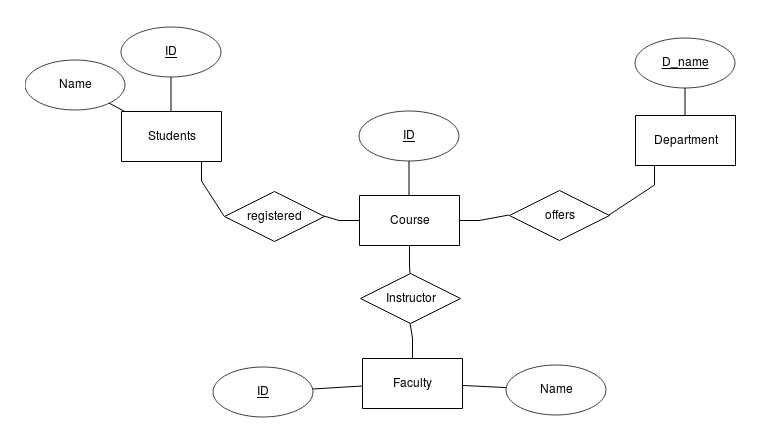
\includegraphics[scale=0.5]{university_ER.png}
\end{figure}

Figure \ref{fig:ER diagram} ER diagram



\end{document}
